\documentclass[a4paper]{article}
\usepackage{titling}
\usepackage{authblk}
\usepackage{fancyhdr}
\usepackage{url}
\usepackage{hyperref}
\usepackage{rsc}
\usepackage{siunitx}
\usepackage{graphicx}
\usepackage{listings}
\usepackage{color}

\definecolor{dkgreen}{rgb}{0,0.6,0}
\definecolor{gray}{rgb}{0.5,0.5,0.5}
\definecolor{mauve}{rgb}{0.58,0,0.82}

\lstset{frame=tb,
  language=Python,
  aboveskip=3mm,
  belowskip=3mm,
  showstringspaces=false,
  columns=flexible,
  basicstyle={\ttfamily},
  numbers=none,
  numberstyle=\tiny\color{gray},
  keywordstyle=\color{blue},
  commentstyle=\color{dkgreen},
  stringstyle=\color{mauve},
  breaklines=true,
  breakatwhitespace=true,
  tabsize=3
}
\DeclareSIUnit\Fahrenheit{\degree F}

\title{Data analysis with Python}
\author[1]{Dr Benjamin J. Morgan}
\author[1,2]{Dr Andrew R. McCluskey}
\affil[1]{Department of Chemistry, University of Bath, email: b.j.morgan@bath.ac.uk}
\affil[2]{Diamond Light Source, email: andrew.mccluskey@diamond.ac.uk}
\setcounter{Maxaffil}{0}
\renewcommand\Affilfont{\itshape\small}

\pagestyle{fancy}
\fancyhf{}
\rhead{CH40208}
\lhead{\thetitle}
\rfoot{\thepage}

\begin{document}
\maketitle

\section*{Aim}
Data analysis is an incredibly important skill in chemistry, however, it is often overlooked. 
In this exercise, you will get an introduction to using Python to fit experimental data, see how model-dependent analysis works in a simple system, and write a Markov chain Monte Carlo algorithm to quantify the inverse uncertainty in your model.
The particular application in this work is the analysis an IR spectra from a mixture of organic species, however, hopefully you will recognise that the methods used herein are generalisable.

\section{Reading in and plotting experimental data}
You have been tasked with determining the relative composition of a mixture of two organic species; namely toluene and benzyl alcohol (Figure~\ref{fig:mole}). 
To do this, you have measured the infrared spectra of the mixture and obtained (from the NIST Chemistry WebBook) the model spectra of the two species in isolation, these can be found in the `IR spectra' folder on Moodle. 
If you download and open the files in the Jupyter Notebook file viewer, you can see the structure of the files. 
You should note that the model datasets (\texttt{benzyl\_alcohol.csv} and \texttt{toluene.csv}) consist of two columns; namely wavenumber ($\bar{\nu}$) and transmittance ($T$), while the measured experimental data (\texttt{mixture.csv}) has a third column that describes the uncertainty in the transmittance. 
%
\begin{figure}[t]
  \centering
  \includegraphics[width=0.5\textwidth]{drawing}
  \label{fig:mole}
  \caption{The organic species in the mixture.}
  \end{figure}
%
\vspace{\baselineskip}
\begin{center}
	\noindent\fbox{%
	    \begin{minipage}{0.9\textwidth}%
	        \vspace{0.15\baselineskip}
			\subsubsection*{Objective 1}
          \begin{itemize}
            \item {Read in the two model datasets, plot them separately using \texttt{matplotlib} including axis labels}
            \item {Read in the experimental dataset, including the third column. Then investigate how this may be plotted using the \texttt{plt.errorbar} functionality} 
          \end{itemize}
          \textbf{Hint}: Googling `matplotlib errorbar' offers some useful instructions on how to use this function, or you can read the documentation with \texttt{plt.errorbar?} in the Jupyter Notebook.
	    \end{minipage}
	}
\end{center}

\section{Interpolation}
Having plotted each of the three datasets (the two models and the experimental), you should be able to identify features present in the experimental data that match those in the models. 
Such as the large feature in the toluene model data, that we can see in the experiment at around \SI{3000}{\per\centi\meter}, and then at higher energy (higher wavenumber), there is a broad feature in the benzyl alcohol data, between \SIrange{3250}{3750}{\per\centi\meter}, that can be found in the experimental data. 
However, you may also note that the values of wavenumber that the spectra have been measured over is not the same between the three datasets, this can be clearly seen by printing the wavenumber for each of the three datasets. 
As we will see, in order to compare the datasets, and to evaluate the composition, we must have the wavenumber values at the same points in the $x$-axis.
This means that interpolation is necessary. 

Interpolation is where we determine new data points within the range of a discrete set of known points. 
Essentially we use what we know about the $x$- and $y$-values and guess at the $y$-values of the different set of $x$ values. 
It is important that the new range of $x$-values is from within the existing range, or else we would be extrapolating (which is often unscientific). 
For the data that you are using, the experimental data lies within the range of the other two datasets, and therefore we will use the wavenumber $x$-values from the experimental dataset and interpolate values for the model data.

To interpolate new $y$-values for the two models, we will use the \texttt{np.interp} function, the documentation for this can be found online (\url{https://docs.scipy.org/doc/numpy/reference/generated/numpy.interp.html}) or by using the \texttt{?} command in the Jupyter Notebook.
Note that this function takes three arguments, in the documentation these are called \texttt{x} which is the new $x$-axis that values should be interpolated for, \texttt{xp} which is the old $x$-axis values, and \texttt{fp} which is the old $y$-axis values. 
This function will return a new set of $y$-axis values, which you should store in a suitably named variable. 

\vspace{\baselineskip}
\begin{center}
	\noindent\fbox{%
	    \begin{minipage}{0.9\textwidth}%
	        \vspace{0.15\baselineskip}
			\subsubsection*{Objective 2}
          \begin{itemize}
            \item {By evaluating the minimum and maximum of each dataset (using the \texttt{np.min} and \texttt{np.max} functions), prove to yourself that the experimental data lays between the model data on the $x$-axis} 
            \item {Create a new variable called \texttt{optimisation\_x} that is the range of $x$-values to be interpolated over (make it equal to the wavenumebr values for the mixture data)}
            \item {Using \texttt{np.interp}, interpolate the toluene and benzyl alcohol data within the values of wavenumber for the mixture}
            \item {Plot the interpolated data to ensure that the interpolation looks similar to the original data}
          \end{itemize}
	    \end{minipage}
	}
\end{center}

\section{Fitting}
Now that all three models have the same $x$-axis, it is possible to begin the procedure of fitting the experimental data to determine the composition of the mixture. 
The function that we will be fitting is the following, 
%
\begin{equation}
  T_{\text{mixture}} = c T_{1} + (1 - c)T_{2},
  \label{equ:model}
\end{equation}
%
where $1$ and $2$ indicate toluene and benzyl alcohol respectively, and $c$ is the fractional composition of toluene (therefore, $1-c$ is the fractional composition of benzyl alcohol as we assume that this is only a two component mixture). 

\vspace{\baselineskip}
\begin{center}
	\noindent\fbox{%
	    \begin{minipage}{0.9\textwidth}%
	        \vspace{0.15\baselineskip}
			\subsubsection*{Objective 3}
          \begin{itemize}
            \item {Write a function that evaluates Equation~\ref{equ:model}, remember to include a docstring}
            \item {Test the function by using it to plot the spectra that would result from a 50:50 mixture of the two components against the experimental mixture data}
          \end{itemize}
	    \end{minipage}
	}
\end{center}

A 50:50 mixture of the two components doesn't do a very good job of modeling the data, therefore we should optimise this value. 
In the optimisation of a model to some experimental data, the value that we typically aim to minimise is some goodness-of-fit metric, such as the $\chi^2$, 
%
\begin{equation}
  \chi^2 = \sum_{i=0}^{N}\bigg[{\frac{y_{\text{model, i}}(c) - y_{\text{exp, i}}}{\text{d}y_{\text{exp, i}}}\bigg]^2},
  \label{equ:chi}
\end{equation}
%
where, $y_{\text{model, i}}(c)$ is the model transmittance at a particular composition, $c$, $y_{\text{exp, i}}$ is the experimentally measured transmittance, $\text{d}y_{\text{exp, i}}$ is the uncertainty in the experimentally measured transmittance, and $N$ is the number of points in the dataset.
The closer the value of $\chi^2$ is to zero, the between the agreement between the model and experiment, in other words we must \emph{minimize} this value.

\vspace{\baselineskip}
\begin{center}
	\noindent\fbox{%
	    \begin{minipage}{0.9\textwidth}%
	        \vspace{0.15\baselineskip}
			\subsubsection*{Objective 4}
          \begin{itemize}
            \item {Write another function that will evaluate the value of $\chi^2$ for a givene $c$, remember to include a docstring}
            \item {Recalling the using of \texttt{scipy.optimize.minimize} from week 3, try and determine the optimum value to minimise the difference between the experiment and the model}
            \item {Store the result of the optimisation and plot the model with the optimised value of $c$ on top of the experimental data to allow you to visually observe the similarity}
          \end{itemize}
	    \end{minipage}
	}
\end{center}

\section{Markov chain Monte Carlo}
You should be aware that all experimental measurements have some associated uncertainty, hence why it is necessary to include error bars on the plot of the mixture data. 
This uncertainty can lead to an \emph{inverse} uncertainty on the model parameters (the $c$ in our model above).
There are a number of methods that we can use to quantify this inverse uncertainty, including the Markov chain Monte Carlo (MCMC) methods introduced here. 

A Markov chain is a \emph{random-walk} through a series of numbers while the Monte Carlo part implies that we will your probability to determine if a \emph{transition} is possible.
In MCMC we start with an initial guess for a variable, which can be taken from a traditional minimisation such as that used in \texttt{scipy.optimize.minimize} and then perturb it by some random amount. 
This random amount is typically obtained based on a step size change with respect to the value of the variable, 
%
\begin{lstlisting}
  perturbation = step\_size * np.random.random() * c,
\end{lstlisting}
%
where, \texttt{c} is the variable to be perturbed.
We then we determine if this random perturbation has improved the agreement to the data (the $\chi^2$-value) or not. 
If it has, we \textbf{accept} this new value for our variable and perform another perturbation. 
If the perturbation does not improve agreement to the data, the new value is \textbf{not} immediately rejected, rather it is only rejected if the probability of this \emph{transition} ($p$) is less than some random number from 0 to 1. 
The probability is found by, 
%
\begin{equation}
  p = \exp{\bigg(\frac{-\chi^2_{\text{new}} + \chi^2}{2}\bigg)},
  \label{equ:prob}
\end{equation}
%
where, $\chi^2$ is the original goodness-of-fit value and $\chi^2_{\text{new}}$ is the goodness of fit after the perturbation. 
This means that it is possible the agreement to get worse overtime, however, the amount by which it can get worse is affected by Equation~\ref{equ:prob}. 
Due to the application of Equation~\ref{equ:prob}, the only values of $\chi^2$ that may be accessed by the Markov chain (these random perturbations on our value) are those that are statistically feasible given the uncertainty on the experimental measurements. 

The algorithm for a typical MCMC sampling process is as follows, 
\begin{enumerate}
  \item {Create an empty list called \texttt{accepted}}
  \item {Evaluate $\chi^2$ for the initial guess of $c$, typically this initial guess would be obtained from a standard optimisation}
  \item {Perturb $c$}
  \item {Calculate $\chi^2_{\text{new}}$ for the new value of $c$}
  \item {Determine the probability of this \emph{transition}, from Equation~\ref{equ:prob}}
  \item {Check if $p \ge n$ where $n$ is a random number from 0 to 1 (this can be obtained from \texttt{np.random.random()}, note that if the new $\chi^2$ is less than the old one then $p > 1$ and therefore this is always accepted}
  \item {If yes, update values of $c$ and $\chi^2$}
  \item {Go to 3 and repeat until the desired number of iterations has been achieved}
\end{enumerate}


\vspace{\baselineskip}
\begin{center}
	\noindent\fbox{%
	    \begin{minipage}{0.9\textwidth}%
	        \vspace{0.15\baselineskip}
			\subsubsection*{Objective 5}
          \begin{itemize}
            \item {Write a function to perform the Markov chain Monte Carlo algorithm outlined above, this function should return the \texttt{accepted} list.}
            \item {Plot a histrogram of the \texttt{accepted} list (using \texttt{plt.hist}), the available values of $c$ should be normally distributed (google a normal distribution and compare)}
            \item {Using the statistical functions in \texttt{numpy}, calculate the \texttt{mean} and standard deviation (\texttt{std}) of this distribution.}
          \end{itemize}
          \textbf{Hint:} Be careful how many iterations you ask you algorithm to perform (you shouldn't ever need more than 1000). Try 100 first to see if it works!
	    \end{minipage}
	}
\end{center}


%\bibliographystyle{rsc}
%\bibliography{handout_1}

\end{document}
